\documentclass[a4paper]{article}
\usepackage[UTF8]{ctex}
\usepackage[a4paper,margin=1in]{geometry}
\usepackage{graphicx}
\usepackage{float}
\usepackage{listings}
\usepackage{booktabs}
\usepackage{hyperref}
\usepackage{fancyhdr}
\usepackage{lastpage}
\usepackage{color}
\usepackage{xcolor}
\usepackage{indentfirst}        % 首段缩进
\setlength{\parindent}{2em}     % 缩进2字符
\usepackage{zhnumber}           % 中文编号
\usepackage[dvipsnames]{xcolor}
\usepackage{amsmath}

% ===== 个人信息与实验信息配置 =====
\newcommand{\projname}{议程管理系统Agenda}
\newcommand{\reporttitle}{实验2-设计文档}
\newcommand{\stuno}{23336179}
\newcommand{\authorname}{马福泉}
\newcommand{\major}{计算机科学与技术}
\newcommand{\adviser}{李文军}
\newcommand{\startdate}{2026年3月}
\newcommand{\labenddate}{2026年4月}
\newcommand{\labroom}{B201}

% ===== 页眉页脚设置 =====
\pagestyle{fancy} 
\fancyhf{}      
\fancyhead[L]{\kaishu \projname}      
\fancyhead[C]{\kaishu \reporttitle}    
\fancyhead[R]{\kaishu \authorname} 
\fancyfoot[C]{第 \thepage 页，共 \pageref{LastPage} 页} 
\renewcommand{\headrulewidth}{0.4pt}
\renewcommand{\footrulewidth}{0pt}

% ===== 代码高亮配置 (适应 Java) =====
\definecolor{NavyBlue}{RGB}{0,0,128}
\lstset{
    language=Java,
    basicstyle=\ttfamily\small,
    commentstyle=\color{gray}\itshape,
    keywordstyle=\color{blue}\bfseries,
    stringstyle=\color{red},
    breaklines=true,
    frame=single,
    numbers=left,
    numberstyle=\tiny\color{gray},
    tabsize=4,
    showstringspaces=false,
    captionpos=b,
    escapeinside={\%}{\%}
}

\begin{document}

% ==================== 封面 ====================
\begin{titlepage}
    \centering
    
    % 若没有校徽图片，可将下面这行注释掉
    
\includegraphics[width=10cm]{img/SYSULogo.png}

    \vspace{1em}
    {\Large \kaishu \projname \par}
    \vspace{3em}

    {\fontsize{36pt}{40pt}\kaishu \selectfont \boldmath \reporttitle\par}
    \vspace{2em}
    \vspace*{\fill}

    \begin{center}
    {\Large
    \makebox[5em][s]{学号}:\underline{\makebox[15em][c]{\kaishu \stuno}}\\[1em]
    \makebox[5em][s]{姓名}:\underline{\makebox[15em][c]{\kaishu \authorname}}\\[1em]
    \makebox[5em][s]{专业}:\underline{\makebox[15em][c]{\kaishu \major}}\\[1em]
    \makebox[5em][s]{指导教师}:\underline{\makebox[15em][c]{\kaishu \adviser}}\\[1em]
    \makebox[5em][s]{起始日期}:\underline{\makebox[15em][c]{\kaishu \startdate}}\\[1em]
    \makebox[5em][s]{结束日期}:\underline{\makebox[15em][c]{\kaishu \labenddate}}\\[1em]
    \makebox[5em][s]{实验地点}:\underline{\makebox[15em][c]{\kaishu \labroom}}
    }
    \end{center}

    \vspace*{\fill}
\end{titlepage}

% ==================== 目录 ====================
\tableofcontents
\newpage

% ==================== 正文 ====================

\section{需求分析与对问题的理解}

\subsection{实验分析}
阅读实验手册的要求，深入分析需求后，我们识别出以下核心需求：

\begin{enumerate}
    \item \textbf{多用户管理复杂性}：系统需要支持多个用户同时注册、登录，并维护各自的会议数据。用户之间存在交互——一个用户可以邀请另一个用户参加会议，这要求系统必须准确追踪每个用户的会议列表。
    
    \item \textbf{业务规则验证的严格性}：会议的创建涉及多重约束条件。首先，发起人和被预约人都必须是已注册用户；其次，两人不能是同一人；最关键的是，\textbf{时间冲突检测}——同一用户在同一时间段内不能有多个会议重叠。这一算法的正确性直接决定系统的可用性。
    
    \item \textbf{终端交互的清晰性}：CLI 系统需要提供直观的命令格式，支持用户注册、会议增删查、批处理等操作，同时给出友好的错误提示。
\end{enumerate}

\subsection{设计约束与扩展性考量}

本实验明确要求系统无需实现数据持久化，采用纯内存操作。然而，这并不意味着可以随意设计。恰恰相反，\textbf{正是因为数据存储方式可能在未来发生变化}（如引入数据库持久化），我们更需要在架构设计上预留解耦空间。

所以选择三层架构：将数据访问逻辑与业务逻辑分离，使得未来替换存储实现时，业务层代码无需任何修改。这正是"面向接口编程"思想的体现。

% ==================== 第二章：面向对象建模与架构设计 ====================
\section{面向对象建模与架构设计}

\subsection{实验结构说明}

本系统采用\textbf{严格三层架构 (3-Tier Architecture)}，将系统划分为三个独立的层次：

\begin{table}[H]
\centering
\begin{tabular}{lll}
\toprule
\textbf{层次} & \textbf{包名} & \textbf{核心职责} \\
\midrule
表示层 & \texttt{agenda.ui} & 命令解析、用户交互、异常捕获与输出 \\
业务逻辑层 & \texttt{agenda.service} & 业务规则验证、时间冲突检测、异常抛出 \\
数据访问层 & \texttt{agenda.storage} & 数据存储、CRUD 操作、单例管理 \\
\bottomrule
\end{tabular}
\caption{三层架构职责划分}
\end{table}

三层架构通过明确的职责划分，实现了"高内聚、低耦合"：

\begin{itemize}
    \item \textbf{下层不依赖上层}：\texttt{Storage} 类完全不知道 \texttt{Command} 的存在，它只提供基础的数据操作方法。这意味着我们可以独立测试数据层，也可以在未来替换存储实现而不影响上层。
    \item \textbf{业务层不包含 UI 逻辑}：\texttt{MeetingService} 中没有任何 \texttt{System.out.println} 语句。当业务校验失败时，它抛出异常而非打印错误信息。这使得业务层可以被不同的界面层复用（如 GUI 或 Web 界面）。
\end{itemize}

\subsection{类图设计}

\begin{figure}[H]
\centering
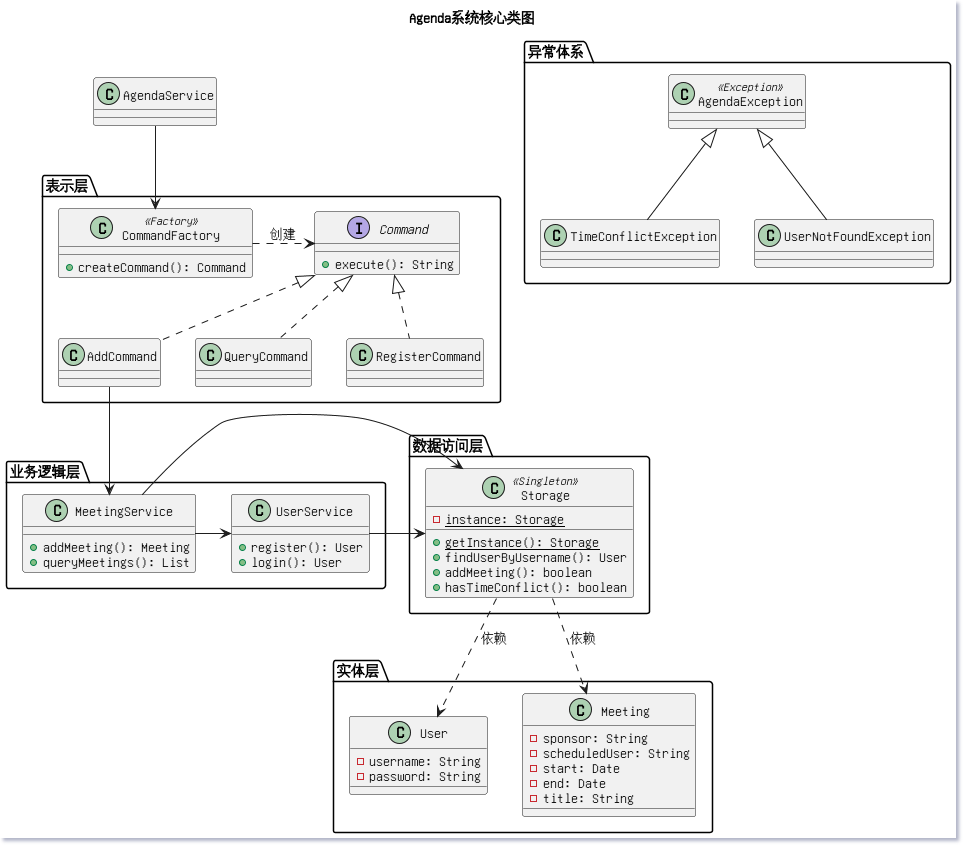
\includegraphics[width=\textwidth]{img/class.png}
\caption{系统核心类图}
\label{fig:class}
\end{figure}

图~\ref{fig:class} 展示了系统的核心类结构。在类图设计中，我们引入了三种 GoF 设计模式，每种模式都有其明确作用：

\subsubsection{单例模式 (Singleton) —— 应用于 Storage 类}

\textbf{为什么？} Agenda 系统是一个多用户系统，所有用户共享同一份数据源。单例模式确保了全局唯一的内存数据源，维护了数据一致性。
实现要点：
\begin{itemize}
    \item 私有构造函数，防止外部直接实例化
    \item 静态私有实例变量
    \item 公有静态 \texttt{getInstance()} 方法，线程安全
\end{itemize}
\subsubsection{命令模式 (Command)与工厂模式 (Factory) —— 应用于 CLI 解析}
\textbf{为什么？} CLI 系统需要支持多种命令（register、add、query、delete 等）。如果不使用命令模式，我们需要在主循环中编写大量的 \texttt{if-else} 或 \texttt{switch-case} 语句。实现了以下优势：
\begin{itemize}
    \item \textbf{开闭原则}：新增命令只需添加新的 \texttt{Command} 实现类，无需修改现有代码
    \item \textbf{单一职责}：每个命令类只负责一个命令的处理逻辑
    \item \textbf{可扩展性}：支持命令的队列化、撤销等高级功能
\end{itemize}

\subsubsection{ 工厂模式 (Factory)}
与上述命令模式配合使用，不再赘述。


\subsection{算法活动图}

添加会议是系统中最复杂的操作，涉及多重校验和时间冲突检测。图~\ref{fig:activity1} 和图~\ref{fig:activity2} 展示了完整的业务流程。

\begin{figure}[H]
    \centering
    % 左侧图片区块
    \begin{minipage}[t]{0.48\textwidth}
        \centering
        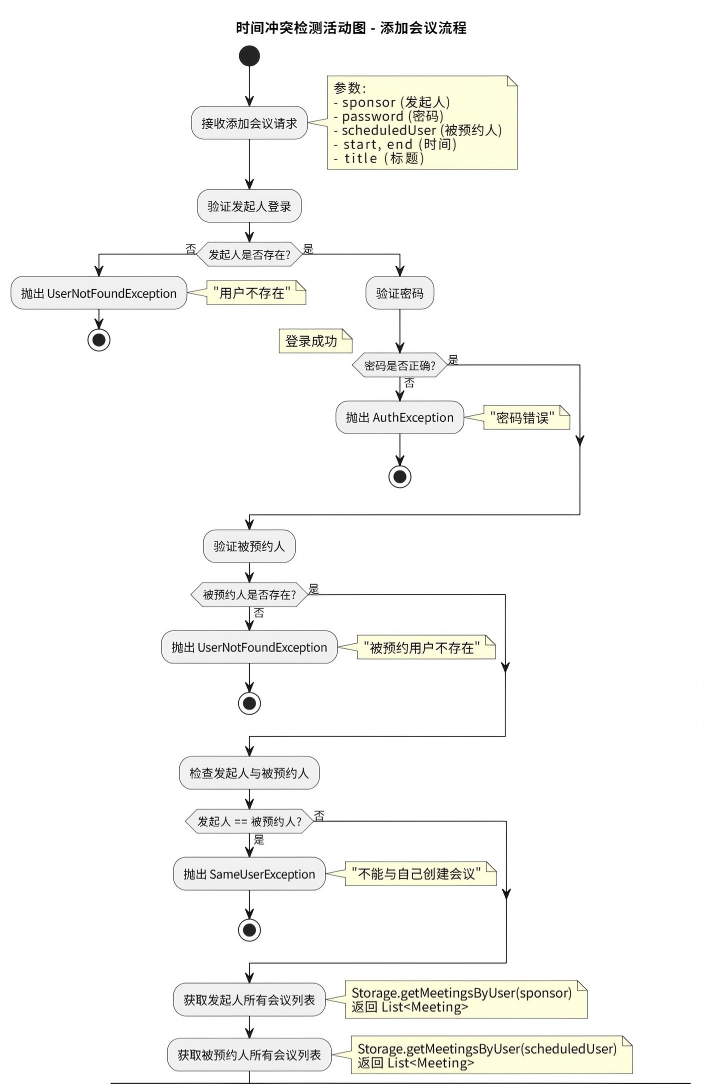
\includegraphics[width=\textwidth]{img/activity1.png}
        \caption{添加会议活动图（上半部分：用户验证）}
        \label{fig:activity1}
    \end{minipage}
    \hfill % 添加弹性空白，将两张图隔开
    % 右侧图片区块
    \begin{minipage}[t]{0.45\textwidth}
        \centering
        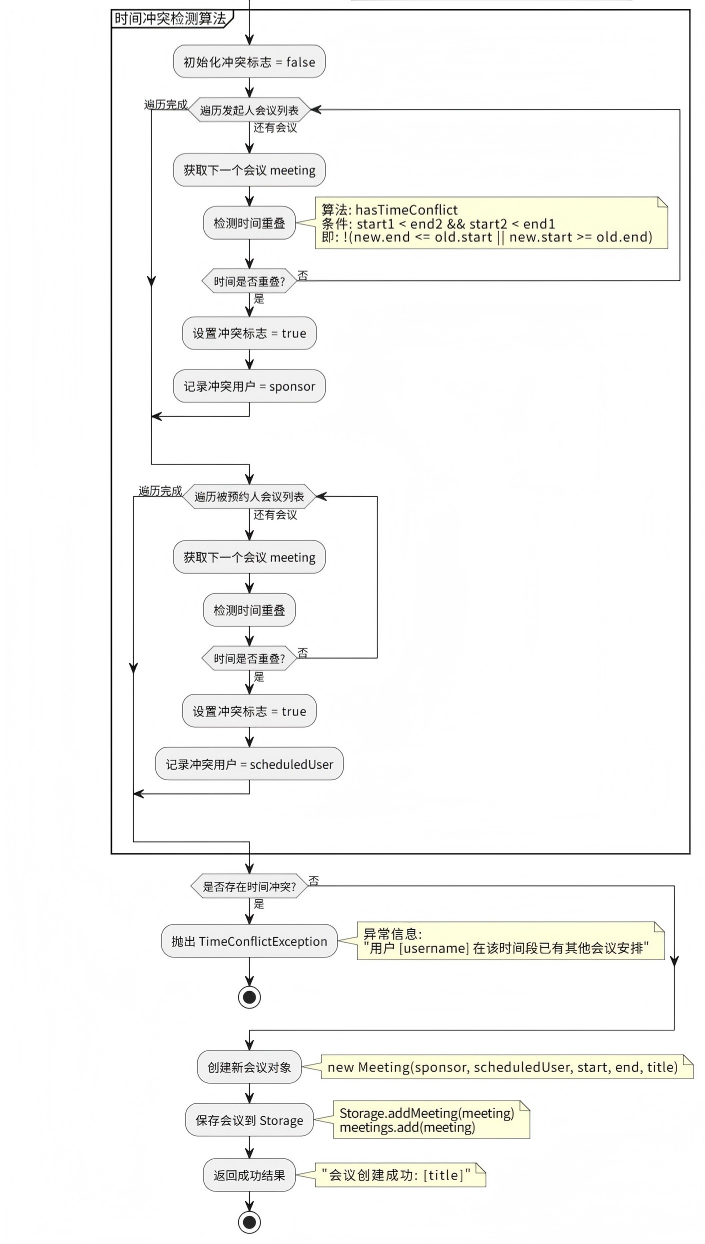
\includegraphics[width=\textwidth]{img/activity2.png}
        \caption{添加会议活动图（下半部分：时间冲突检测与创建）}
        \label{fig:activity2}
    \end{minipage}
\end{figure}

从活动图可以看出，业务层按照严格的顺序执行校验：
\begin{enumerate}
    \item \textbf{发起人存在性校验}：调用 \texttt{UserService.login()} 验证用户名和密码
    \item \textbf{被预约人存在性校验}：确保被邀请的用户已注册
    \item \textbf{相同用户检查}：发起人不能邀请自己
    \item \textbf{时间冲突遍历检测}：遍历两人的所有会议，检测时间重叠
\end{enumerate}

\subsection{添加会议交互时序图}
\begin{figure}[H]
\centering
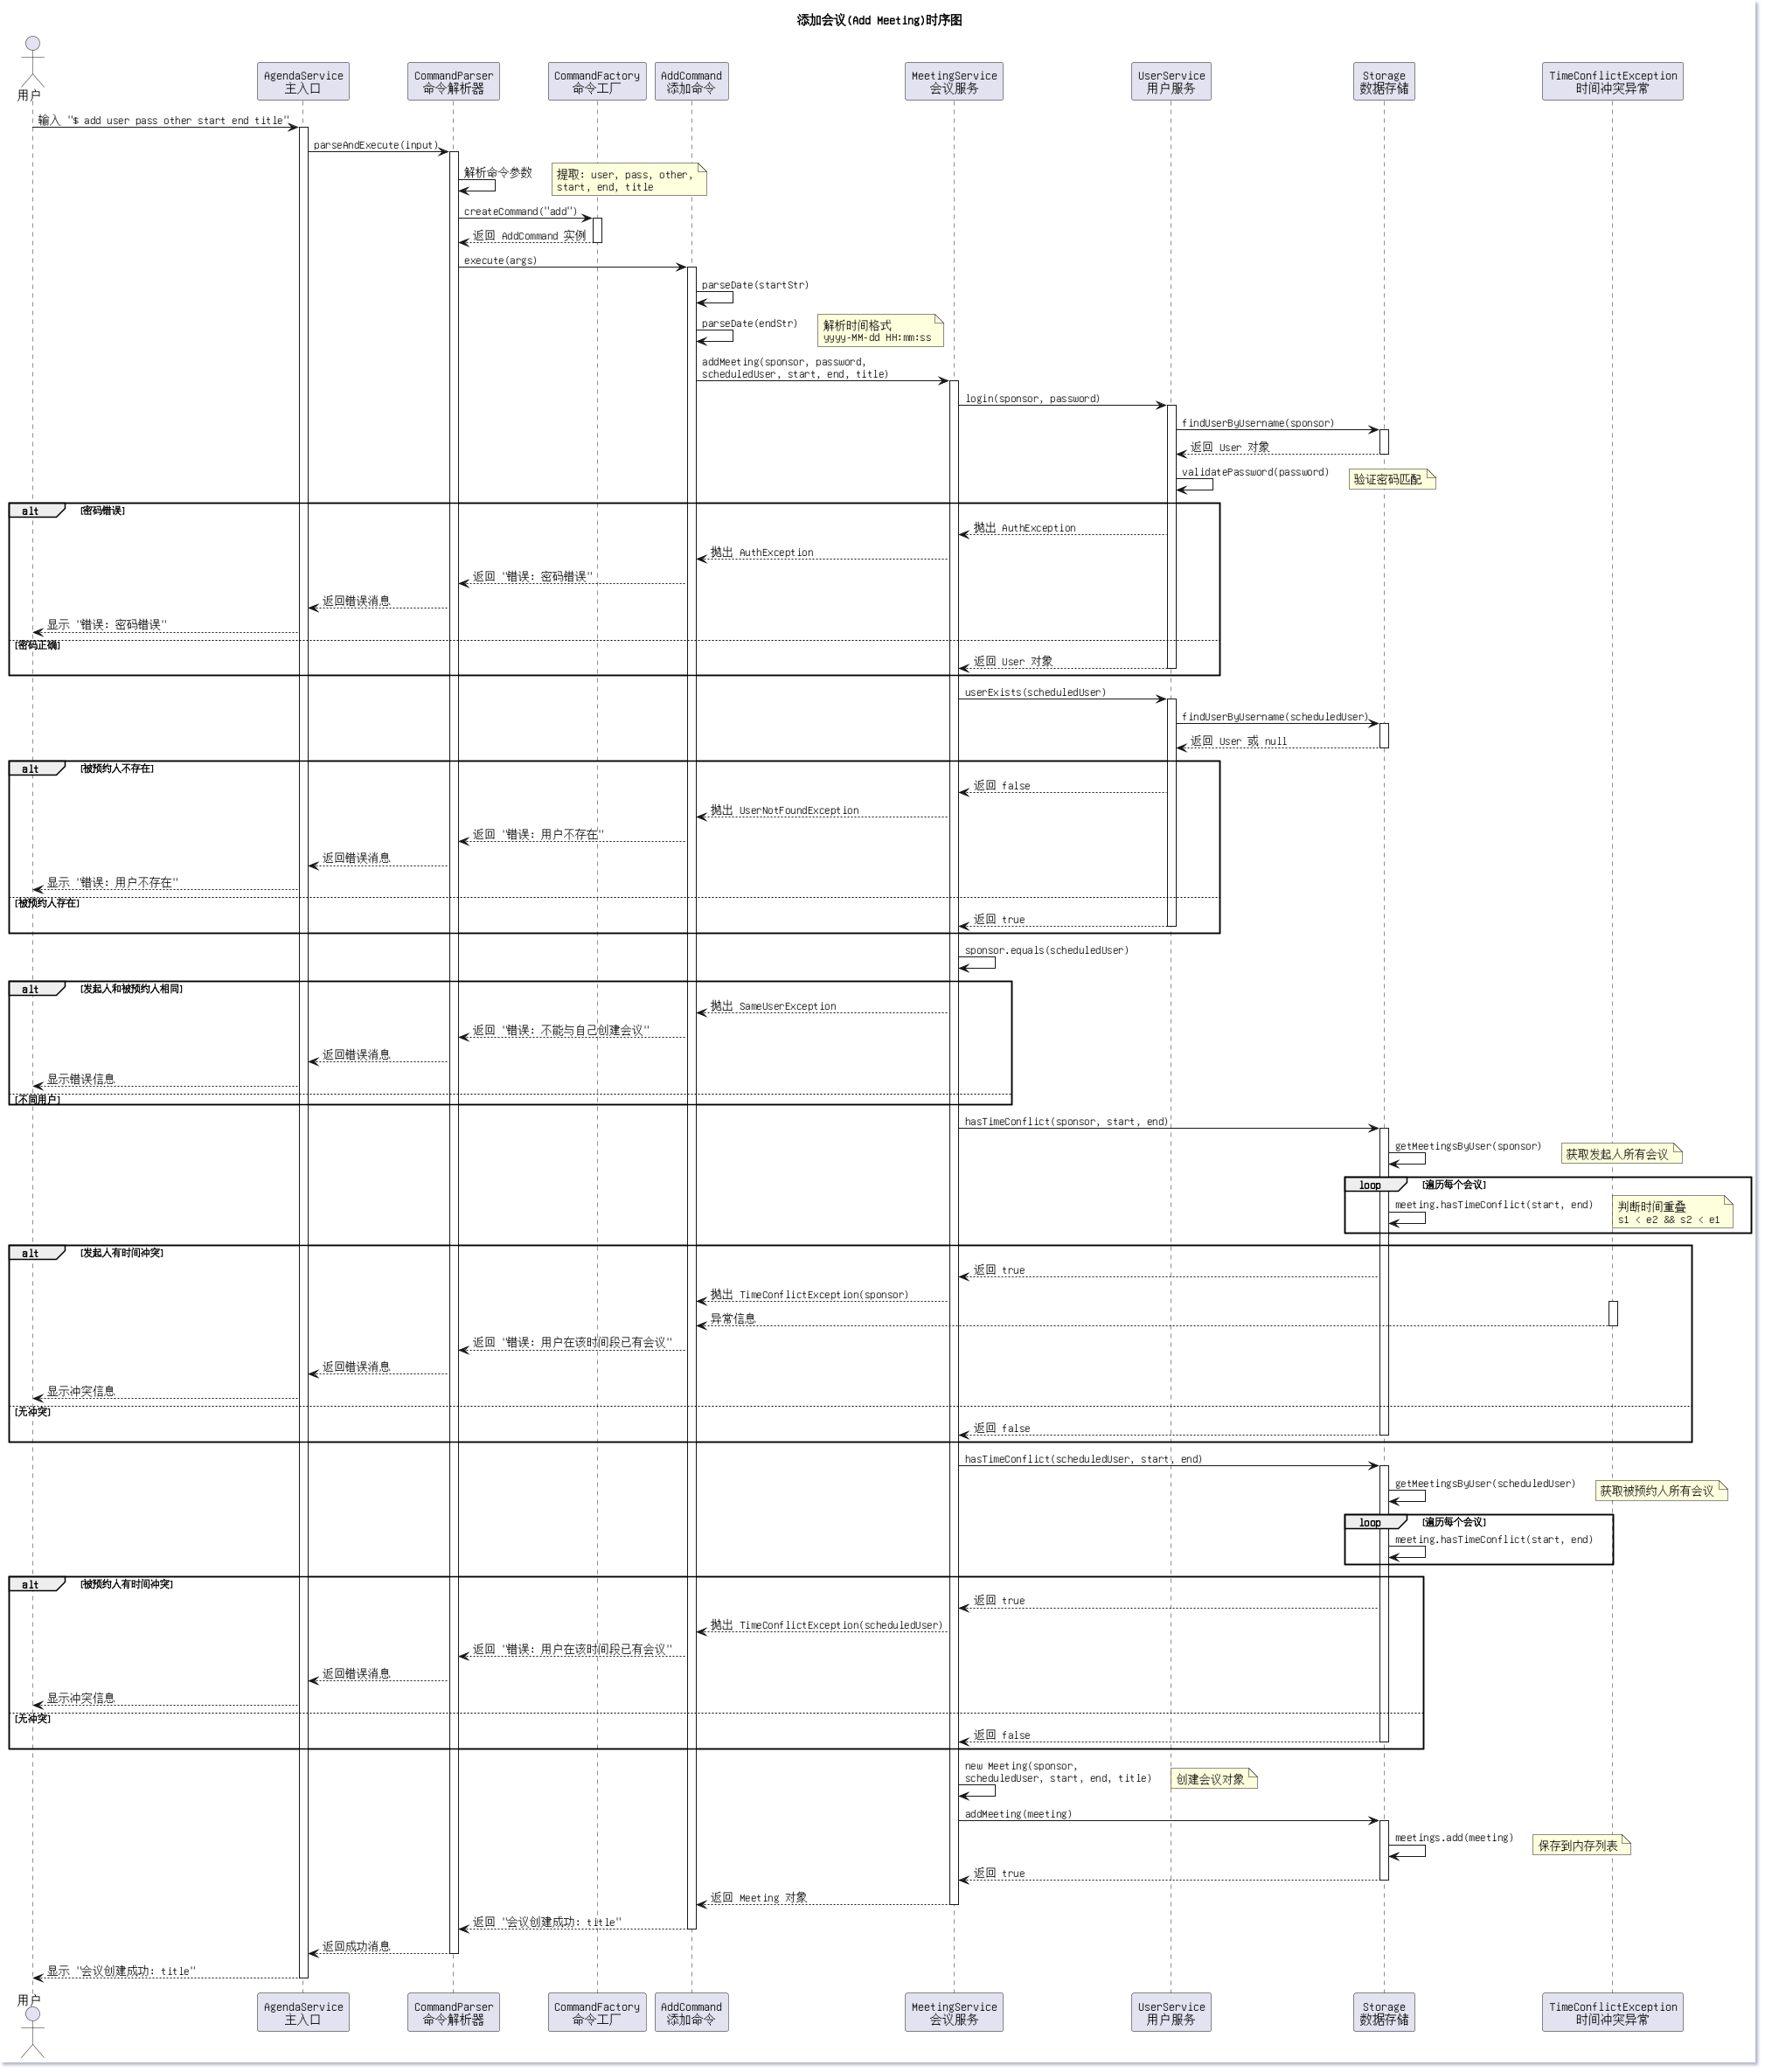
\includegraphics[width=\textwidth]{img/sequence.png}
\caption{添加会议时序图}
\label{fig:sequence}
\end{figure}
\textbf{注：} 此时序图由工具根据源码自动生成，涵盖了从 UI 到 Storage 的完整调用链路。因跨层级交互链路较长，图片整体尺寸偏小，特在此展示系统各层调用的宏观时序关系：
\begin{enumerate}
    \item 用户输入命令，\texttt{AgendaService} 接收并传递给 \texttt{CommandParser}
    \item \texttt{CommandParser} 解析命令，通过 \texttt{CommandFactory} 创建 \texttt{AddCommand}
    \item \texttt{AddCommand} 调用 \texttt{MeetingService.addMeeting()}
    \item \texttt{MeetingService} 依次调用 \texttt{UserService} 和 \texttt{Storage} 完成验证和存储
\end{enumerate}

% ==================== 第三章：算法与设计分析 ====================
\section{算法与设计分析}

\subsection{时间重叠 (Overlap) 算法的数学化简}

时间冲突检测是本系统最核心的算法。给定两个时间段 $[s_1, e_1]$ 和 $[s_2, e_2]$，如何判断它们是否存在重叠？

\subsubsection{朴素思路}

最容易想到的方法是列举所有重叠情况：
\begin{itemize}
    \item 时间段 1 完全包含时间段 2
    \item 时间段 2 完全包含时间段 1
    \item 时间段 1 的后半部分与时间段 2 的前半部分重叠
    \item 时间段 1 的前半部分与时间段 2 的后半部分重叠
\end{itemize}

这种方法需要判断 4 种情况，代码冗长且容易出错。

\subsubsection{逆向思维：判断"不重叠"}

让我们换一个角度思考：两个时间段\textbf{不重叠}的条件是什么？

显然，不重叠只有两种情况：
\begin{itemize}
    \item 时间段 1 完全在时间段 2 之前：$e_1 \leq s_2$
    \item 时间段 1 完全在时间段 2 之后：$s_1 \geq e_2$
\end{itemize}

因此，不重叠的条件是：
\begin{equation}
e_1 \leq s_2 \lor s_1 \geq e_2
\end{equation}

\subsubsection{应用德摩根定律}

根据德摩根定律：
\begin{equation}
\neg(A \lor B) = \neg A \land \neg B
\end{equation}

对不重叠条件取反，即得到重叠条件：
\begin{equation}
\neg(e_1 \leq s_2 \lor s_1 \geq e_2) = s_1 < e_2 \land s_2 < e_1
\end{equation}

这就是最终的时间冲突检测算法：
\begin{lstlisting}
public boolean hasTimeConflict(Date otherStart, Date otherEnd) {
    return start.before(otherEnd) && otherStart.before(end);
}
\end{lstlisting}

\textbf{算法优势}：
\begin{itemize}
    \item 仅需两次比较运算，时间复杂度 $O(1)$
    \item 逻辑简洁，不易出错
    \item 避免了繁琐的边界情况枚举
\end{itemize}

\subsection{扩展性优势}

命令模式的引入为系统带来了极佳的扩展性。假设未来需要新增 \texttt{help} 命令或 \texttt{unregister} 命令，只需：

\begin{enumerate}
    \item 创建新的命令类，实现 \texttt{Command} 接口：
\begin{lstlisting}
public class HelpCommand implements Command {
    public String execute(String[] args) {
        return "可用命令: register, add, query, ...";
    }
    public String getName() { return "help"; }
    public String getUsage() { return "help - 显示帮助"; }
}
\end{lstlisting}

    \item 在 \texttt{CommandFactory} 中注册新命令：
\begin{lstlisting}
case "help":
    return new HelpCommand();
\end{lstlisting}
\end{enumerate}

整个过程\textbf{完全不需要修改}主循环 \texttt{AgendaService.start()} 或命令解析器 \texttt{CommandParser}，完美符合开闭原则（对扩展开放，对修改关闭）。

\subsection{程序的健壮性}

系统的健壮性通过\textbf{自定义异常体系}实现。我们设计了层次化的异常结构：

\begin{itemize}
    \item \texttt{AgendaException}：基础异常类，继承自 \texttt{Exception}
    \item \texttt{UserNotFoundException}：用户不存在
    \item \texttt{TimeConflictException}：时间冲突
    \item \texttt{AuthException}：认证失败
    \item \texttt{SameUserException}：发起人与被预约人相同
    \item \texttt{MeetingNotFoundException}：会议不存在
\end{itemize}

\begin{lstlisting}
// MeetingService.java - 业务层只抛异常
public Meeting addMeeting(...) throws TimeConflictException {
    if (storage.hasTimeConflict(sponsor, start, end)) {
        throw new TimeConflictException(sponsor);
    }
    // 正常逻辑
}

// AddCommand.java - UI层捕获并处理
public String execute(String[] args) {
    try {
        meetingService.addMeeting(...);
        return "会议创建成功";
    } catch (TimeConflictException e) {
        return "错误: " + e.getMessage();
    }
}
\end{lstlisting}
优势：
\begin{enumerate}
    \item 业务层代码专注于业务逻辑，可读性强
    \item 异常信息准确，便于调试
    \item UI 层可以灵活决定错误信息的展示方式
\end{enumerate}

% ==================== 第四章：总结 ====================
\section{总结}
\begin{enumerate}
    \item \textbf{架构设计的重要性}：三层架构的严格划分，使得各层职责清晰，代码易于维护和测试。下层不依赖上层的设计原则，为未来的扩展（如引入数据库持久化）预留了空间。
    
    \item \textbf{设计模式的价值}：单例模式保证了数据一致性，命令模式实现了请求的参数化，工厂模式集中了对象创建逻辑。这些模式的合理运用，使系统具备了良好的扩展性。
    
    \item \textbf{算法设计的优雅性}：时间冲突检测算法通过数学化简，从繁琐的边界枚举简化为两次比较运算，体现了"简洁即美"的工程哲学。
    
    \item \textbf{异常处理的规范性}：层次化的异常体系，配合"业务层抛出、UI层捕获"的模式，实现了正常逻辑与异常处理的清晰分离。
\end{enumerate}
通过本次实验，我深刻体会到：优秀的软件设计不仅仅是实现功能，更重要的是为变化做好准备。三层架构、设计模式、异常处理机制，这些看似增加了代码量的设计，实际上是在为系统的长期演进奠定基础。

\end{document}